% !TEX root = ./Vorlesungsmitschrift DIFF 2.tex  
\lecture{Mo 27.04. 10:15}{}
\begin{lemma}[Cauchy-Kriterium für gleichmäßige Konvergenz]\label{cauchy_kriterium_gleichmaessige_konvergenz}\hfill
    \begin{eigenschaftenenumerate}
        \item Sei \( (X,d_x)\) metrischer Raum, sei \( (Y,d_Y)\) ein \emph{vollständiger} metrischer Raum. Sei \( f_n\maps X\to Y\) Folge von Funktionen. Dann konvergiert \( f_n\) gegen \( f\) bezüglich
        \begin{align*}
            d_{\sup}(h,g)\definedas \sup_{t\in X} \underbrace {d_{Y}(f(t),g(t))}_{\in \reals } \quad h,g\maps X\to Y
        \end{align*}
        \tiff \tforall \( \varepsilon>0\) \texists \( N=N(\varepsilon)\in \naturals \) \sd
        \begin{align*}
            d_Y(f_n(t),f_m(t))<\varepsilon \quad \forall t\in X\logicspace n,m\geq N(\varepsilon).\tag{*}\label{eq:cauchy_kriterium_gleichmaessige_konvergenz}
        \end{align*} 
        \begin{notation*}
            Man spricht von \emph{gleichmäßiger Konvergenz}.
        \end{notation*}
        \minisec{Beachte:} Der wesentliche Punkt in \eqref{eq:cauchy_kriterium_gleichmaessige_konvergenz} ist, dass \( N\) unabhängig von \( t\) gewählt werden kann.
        
        \begin{proof}
            Wir stellen zunächst fest, dass \( d_{\sup}\) auf
            \begin{align*}
                \mathcal{F}\definedas \Set{f \maps X\to Y|\text{Für je zwei Funktionen gilt: }d_{\sup}(f_1,f_2)<\infty}
            \end{align*} 
            eine Metrik definiert (auch wenn \( Y\) nicht vollständig ist).
            \begin{proofdescription}
                \item[\ref{metrik:nicht_ausgeartet}] \begin{align*}
                    &d_{\sup}(f,g)=0\\
                    \iff &d_{Y}(f(t),g(t))=0 \logicspace \forall t\in X\\
                    \explain{d_Y\text{ ist Metrik}}{\iff} &f(t)=g(t)\logicspace \forall t\in X
                \end{align*}
                \item[\ref{metrik:symmetrisch}]
                \begin{align*}
                    d_{\sup}(f,g)=\sup d_Y(f(t),g(t))=\sup d_Y(g(t),f(t))=d_{\sup}(g,f)
                \end{align*} 
                \item[\ref{metrik:dreiecksungleichung}] \begin{align*}
                    d_{\sup}(f,g)
                    \begin{aligned}[t]
                        &=\sup \underbrace{d_Y(f(t),g(t))}_{\mathclap{\leq d_Y(f(t),h(t))+d_Y(h(t),g(t))}}\\
                        &\leq \sup d_Y(f(t),h(t))+\sup d_Y(h(t),g(t))\\
                        &=d_{\sup} (f,h)+d_{\sup} (h,g)
                    \end{aligned}
                \end{align*}
            \end{proofdescription}
            \minisec{Zum Beweis der Behauptung:}
            \begin{proofdescription}
                \item[\hin] \begin{align*}
                    \sup_t d_Y(f_n(t),f(t))<\varepsilon\quad \forall n\geq N(\varepsilon)
                \end{align*}
                impliziert
                \begin{align*}
                    d_Y(f_n(t),f(t))<\varepsilon\quad \forall t\in X\logicspace \forall n\geq N(\varepsilon),
                \end{align*} 
                somit für \emph{alle} \( t\in X\)
                \begin{align*}
                    d_Y(f_n(t),f_m(t))\begin{aligned}[t]
                        &\underset{\mathclap{\triangle(d_Y)}}{\leq} d_Y(f_n(t),f(t))+d_Y(f(t),f_m(t))\\
                        &<2\varepsilon \quad \forall n,m\geq N(\varepsilon)
                    \end{aligned}
                \end{align*} 
                \item[\rueck] Gelte \eqref{eq:cauchy_kriterium_gleichmaessige_konvergenz}. Dann ist für jedes \( t\in X\), dass \( (f_n(t))_n\) ist Cauchy-Folge in \( Y\).  
                
                Vollständigkeit von \( Y\) \timplies \( (f_n(t))_n\) konvergiert. Setze \( f(t)\definedas \lim\limits_{n \goesto \infty} f_n(t)\).
                
                Wir zeigen \( f_n\) konvergiert bezüglich \( d_{\sup}\) gegen \( f\). Sei also \( \varepsilon>0\). Wähle in \eqref{eq:cauchy_kriterium_gleichmaessige_konvergenz} \( m\geq N(\varepsilon)\) fest. Dann gilt für \emph{alle} \( t\):
                \begin{align*}
                    \varepsilon \begin{aligned}[t]
                        &\geq \lim\limits_{n \goesto \infty} d_Y(f_n(t),f_m(t))\\
                        &\explain{d_Y\text{ ist stetig}}{=} d_Y(f(t),f_m(t)).
                    \end{aligned}
                \end{align*}
                Das gilt für alle \( m\geq N(\varepsilon)\), \tforall \( t\), also auch für das Supremum \timplies \Beh.
            \end{proofdescription}
            
            
        \end{proof}
        \item \label{gleichmaessige_konvergenz_stetigkeit}Seien \( X,Y\) metrische Räume, \( (f_n)_n\) eine Folge \emph{stetiger} Funktionen \( f_n\maps X\to Y\), die gleichmäßig konvergiere. Dann ist die Grenzfunktion \( f\maps X\to Y\).
        \begin{proof}
            Sei \( a\in X\). Sei \( \varepsilon>0 \). Gleichmäßige Konvergenz \timplies \texists \( N=N(\varepsilon)\in \naturals \) \sd 
            \begin{align*}
                d_Y(f(t),f_n(t))<\varepsilon\quad \forall t\in X\logicspace \forall n\geq N
            \end{align*} 
            \( f_n\) stetig in \( a\) \timplies \texists \( \delta > 0 \) \sd
            \begin{align*}
                &d_Y(d_N(t),f_N(a))<\varepsilon\quad \forall t\text{ mit } d_X(t,a)<\delta\\
                \implies &d_Y(f(t),f(a))\begin{aligned}[t]
                    &\underset{\triangle}{\leq}d_Y(f(t),f_N(t))+d_Y(f_N(t),f_N(a))+d_Y(f_N(a),f(a))\\
                    &<3\varepsilon\quad \forall t\text{ mit }d_X(t,a)<\delta.
                \end{aligned}
            \end{align*}
            
        \end{proof}
         
    \end{eigenschaftenenumerate}
        
\end{lemma}
\begin{folgerung*}
    \begin{align*}
        (C(\explain{\text{Stellt man diese Bedingung, ist automatisch garantiert, dass \( d_{\sup}(f_1,f_2)=\sup_{t\in \rinterval{a}{b}}\abs{f_1(t)-f_2(t)}<\infty \)}}{\interval{a}{b}},\reals),d_{\sup})
    \end{align*}, \( D\subset \reals \), ist vollständig.  
\end{folgerung*}
\begin{proof}
    Sei \( (f_n)_n\) Cauchy-Folge in \( C(D,\reals )\) bezüglich \( d_{\sup}\), \dh zu \( \varepsilon>0 \) \texists \( N=N(\varepsilon)\) \sd
    \begin{align*}
        &d_{\sup}(f_n,f_m)<\varepsilon\quad \forall n,m\geq N(\varepsilon)\\
        \implies &d_Y(f_n(t),f_m(t))=\abs{f_n(t)-f_m(t)}<\varepsilon \quad \forall n,m\geq N(\varepsilon)\logicspace \forall t\in D. 
    \end{align*} 
    \( \reals \) ist vollständig
    \begin{proofdescription}
        \item[\( \overset{\text{\ref{cauchy_kriterium_gleichmaessige_konvergenz}}}{\implies}\)] \( (f_n)_n\) konvergiert bezüglich \( d_{\sup}\) gegen seinen punktweisen Grenzwert
        \begin{align*}
            f(t)\definedas \lim\limits_{n \goesto \infty} f_n(t)\quad (\text{Konvergenz in \( \reals \)})
        \end{align*}   
        \item[\( \overset{\text{\ref{gleichmaessige_konvergenz_stetigkeit}}}{\implies}\)] \( t\mapsto f(t)\) ist stetig. 
    \end{proofdescription}
    
\end{proof}
\section*{Stetige Abbildungen auf metrischen Räumen}
\begin{lemma}\label{metrische_raeume_komposition_stetig}
    Seien \( X,Y,Z\) metrische Räume, \( f\maps X\to Y\), \( g\maps Y\to Z\), \( f(X)\subset Y\). Ist \( f\) stetig in \( a\in X\) und \( g\) stetig in \( b=f(a)\in \tilde{Y} \), so ist \( g\circ f\maps X\to Z\) stetig in \( a\).
\end{lemma}
\begin{proof} (Über Folgenstetigkeit, \thref{stetigkeit:folgenkonvergenzkriterium})
    Sei \( x_n\goesto a\) \timplies \( \lim f(x_n)=(a)=b\) und \( \lim g(f(x_n))=g(b)=g(f(a))\) \timplies \( \lim g\circ f(x_n)=g\circ f(a)\).   
    
\end{proof}
\begin{definition}
    Auf dem \( \reals^n\) ist durch
    \begin{align*}
        d_{\max}(x,y)\definedas \max_{i\in \Set{1,\ldots,n}}\abs{x_i-y_i}. 
    \end{align*}
    eine Metrik definiert.
\end{definition}
\begin{bemerkungen*}
    \begin{enumerate}
        \item \( d_{\max}(x,y)=d_{\sup}(x,y)\), fasst man \( x\) und \( y\) als Abbildungen
        \begin{align*}
            x\maps \Set{1,\ldots, n}\to \reals 
        \end{align*} 
        auf, \( x(i)=x_i\).
        \item \label{d_max:folgenkonvergenz}Eine Folge \( (x_m)_m\subset \reals^n \), \( x_m=(x_m^1,\ldots, x_m^n)\) konvergiert bezüglich \( d_{\max}\) \tiff Alle \emph{Komponentenfolgen} \( (x_m^i)_m\quad (1\leq i\leq n)\) konvergieren in \( \reals \).
        \begin{proof}
            \begin{proofdescription}
                \item[\hin] Zu \( \varepsilon>0\) \texists \( N\) \sd \( \max \abs{x_m^i-a_m^i}<\varepsilon\quad \forall m\geq N \).
                \item[\rueck] Zu \( \varepsilon>0\) \texists \( N_i\) \sd \( \abs{x_m^i-a_m^i}<\varepsilon \quad \forall m\geq N_i\)
                \begin{align*}
                    \implies \max_i \abs{x_m^i-a_m^i}<\varepsilon\quad \forall m\geq N=\max\Set{N_1,\ldots, N_n}. 
                \end{align*} 
            \end{proofdescription}
            
            
        \end{proof}
        
        \item Es folgt: \( (\reals^n, d_{\max})\) ist \emph{vollständig}.
        \item \( B_\varepsilon(a)\) bezüglich dieser Metrik:
        \begin{align*}
            \Set{x\in \reals ^n |\max_{i\in \Set{1,\ldots, n}}\abs{x_i-a_i}<\varepsilon},
        \end{align*}
        Würfel mit Seitenlängen \( 2\varepsilon\) um \( a\).
        \begin{figure}[H]
            \centering
            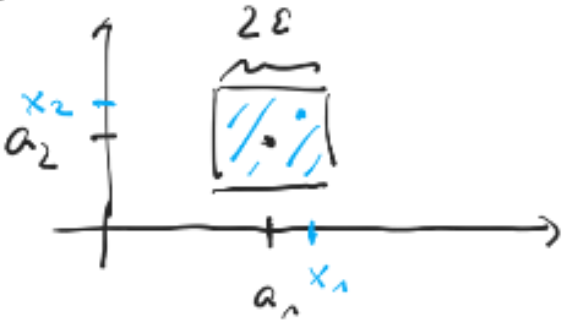
\includegraphics[width=0.3\linewidth]{figures/d_max_ball}
            \label{fig:d_max_ball}
        \end{figure}
        
    \end{enumerate}
\end{bemerkungen*}

\begin{lemma}\label{d_max:metrischer_raum_zu_r_stetigkeit:komponenten}
    Sei \( (X,d)\) metrischer Raum. Sei \( @rr
    ^n\) mit \( d_{\max}\) versehen. Eine Abbildung \( f\maps X\to \reals ^n\), \( f=(f_1,\ldots, f_n)^T\), 
    \begin{align*}
        f(y)=(f_1(y),\ldots, f_n(y))^T\in \reals^n, y\in X.
    \end{align*}   
    \( f_i\maps X\to \reals \), \( i\in \Set{1,\ldots,n}\), \enquote{\emph{Komponenten-Funktionen}}, ist genau dann stetig in \( a\in X\), falls alle \( f_i\) stetig in \( a\) sind.
\end{lemma}
\begin{proof}
    Mit Folgenstetigkeit direkt aus Bemerkung~\ref{d_max:folgenkonvergenz}. Hier nochmals mit \( \varepsilon\)-\( \delta\)-Kriterium.
    \begin{notation*}
        \( \underline{n}=\Set{1,\ldots,n}\). 
    \end{notation*}
    \begin{proofdescription}
        \item[\hin] Sei also \( f\maps X\to \reals^n\) stetig in \( a\). Sei \( \varepsilon>0\). Dann \texists \( \delta>0\) \sd
        \begin{align*}
            &\max_{i\in \underline{n}}\abs{f_i(y)-f_i(a)}<\varepsilon\forall y\in \explain{\text{bezüglich }d}{B_\delta(a)}\\
            \implies &\abs{f_i(y)-f_i(a)}<\varepsilon\quad \forall y\in B_\delta(a)\logicspace \forall i\in \underline{n}\\
            \implies &f_i\text{ sind stetig in }a.
        \end{align*}  
        \item[\rueck] Seien also die \( f_i\maps X\to \reals \), \( i\in \underline{n}\), stetig in \( a\). Sei \( \varepsilon>0\). Dann \texists \( \delta_i>0\) \sd 
        \begin{align*}
            \abs{f_i(y)-f_y(a)}<\varepsilon\quad \forall y\in B_{d_i}(a)\subset X. 
        \end{align*}   
        Wähle \( d\definedas \min \Set{\delta_1,\ldots,\delta_n}\). Dann ist
        \begin{align*}
            \max_{i\in \underline{n}}\abs{f_i(y)-f_i(a)}<\varepsilon\quad \forall y\in B_d(a). 
        \end{align*} 
    \end{proofdescription}
\end{proof}
\begin{lemma}\label{d_max:operationen_stetig}
    Folgende Abbildungen sind stetig:
    \begin{align*}
        \operatorname{add}\maps \reals^2\to \reals,\logicspace \operatorname{add}(x,y)=x+y\\
        \operatorname{mult}\maps \reals^2\to \reals,\logicspace \operatorname{mult}(x,y)=x\cdot y\\
        \operatorname{quot}\maps \reals \times\equalto{\reals \setminus\zeroset}{\reals^{*}}\to \reals,\logicspace \operatorname{quot}(x,y)=x/y.
    \end{align*}
    Hierbei sei \( \reals^2\), \( \reals \times\reals^{*}\), mit \( d_{\max}\) versehen.
\end{lemma}
\begin{proof}
    Sei \( ((x_m,y_m))_m\subset \reals^2\) mit \( (x_m,y_m)\goesto (x,y)\) (bezüglich \( d_{\max}\))
    \begin{align*}
        \underset{\text{Bem~\ref{d_max:folgenkonvergenz}}}{\implies} &x_m\goesto x\text{ und }x_m\goesto y\text{ in }\reals \\
        \implies& \lim (x_m+y_m)=x+y\\
        &\lim (x_m\cdot y_m)=x\cdot y\\
        &\lim (x_m/y_m)=x/y\quad (\text{falls }y_m \neq 0,y\neq 0).
    \end{align*}
    
\end{proof}
\begin{folgerung*}
    Sei \( (X,d)\) metrischer Raum. Seien \( f,g\maps X\to \reals \) stetig. Dann sind auch
    \begin{align*}
        f+g&\maps X\to \reals,\logicspace  (f+g)(x)=f(x)+g(x) \text{ und}\\
        g\cdot g&\maps X\to \reals,\logicspace (f\cdot g)(x)=f(x)\cdot g(x)
    \end{align*}
    stetig. Gilt \( g(x)\neq 0 \quad \forall x\in X\), so ist auch
    \begin{align*}
        f/g\maps X\to \reals, (f/g)(x)=f(x)/g(x)
    \end{align*}
    stetig.
\end{folgerung*}
\begin{proof}
    \begin{align*}
        \ref{d_max:metrischer_raum_zu_r_stetigkeit:komponenten} \implies \begin{pNiceMatrix} f \\ g \end{pNiceMatrix}\maps X\to \reals^2, \begin{pNiceMatrix} f \\ g \end{pNiceMatrix}(x)=\begin{pNiceMatrix} f(x) \\ g(x) \end{pNiceMatrix}  
    \end{align*}
    ist stetig. 

    Es ist
    \begin{align*}
        f+g&=\operatorname{add}\circ \begin{pNiceMatrix} f \\ g \end{pNiceMatrix}\\
        f+g&=\operatorname{mult}\circ \begin{pNiceMatrix} f \\ g \end{pNiceMatrix}\\
        f/g&=\operatorname{quot}\circ \begin{pNiceMatrix} f \\ g \end{pNiceMatrix}
    \end{align*}
    Mit \ref{d_max:operationen_stetig} und \ref{metrische_raeume_komposition_stetig} folgt die Behauptung.
\end{proof}
\begin{beispiel*}
    Polynomische Funktionen \( \reals^n\to \reals \) 
    \begin{align*}
        x\mapsto \sum\limits_{0\leq k_i\leq r}c_{\underbrace{k_1\cdots k_n}_{\in \reals}}x_1^{k_1}\cdots x_n^{k_n} 
    \end{align*}
    sind stetig.
\end{beispiel*}
\begin{bemerkung}
    Wir werden später sehen, dass die Aussage in \ref{d_max:operationen_stetig} auch gilt, wenn man den \( \reals ^2\) \zb mit dem Euklidischen Abstand versieht.
\end{bemerkung}
\section*{Kompaktheit}
\begin{definition}
    Sei \( (X,d)\) metrischer Raum, \( M\subset X\). Eine \emph{offene Überdeckung von \( M\)} ist eine Familie \( (U_i)_{i\in I}\) von offenen Teilmengen \( U_i\subset X\) mit \( M\subset \bigcup\limits_{i\in I}U_i\) (\( I\) eine beliebige Indexmenge).   
\end{definition}
\begin{definition}
    \( M\subset X\) heißt \emph{kompakt}, falls es zu \emph{jeder} offenen Überdeckung von \( \bigcup_{i\in I} U_i \) von \( M\) \emph{endlich} viele Indizes \( i_1,\ldots, i_N\) gibt \sd
    \begin{align*}
        M\subset U_{i_1}\cup \cdots \cup U_{i_N}.
    \end{align*} 

    \begin{achtung*}
        Ein nicht-kompakter raum kann eine endliche Überdeckung \( U_1\cup \cdots \cup U_N\) besitzen. Die Aussage der Definition ist, dass man aus \emph{jeder} offenen Überdeckung endlich viele offene Mengen wählen kann, die \( M\) noch ganz überdecken!
    \end{achtung*}
\end{definition}
\begin{beispiele}
    \begin{enumerate}
        \item \( \interval{a}{b} \) ist kompakt (Beweis später).
        \item \( \ointerval{a}{b} \) ist nicht kompakt (obwohl etwa \( \ointerval{a}{b} \) eine endliche offene Überdeckung ist!)
        \begin{proof}
            \begin{align*}
                U_j=\ointerval{a+\frac{1}{j}}{b},\logicspace j\geq 1\\
                \bigcup_j U_j=\ointerval{a}{b} 
            \end{align*}
            aber ed gibt \emph{kein} \( N\) \sd
                \( \bigcup\limits_{j=1}^{N}U_j\supset \ointerval{a}{b} \), denn \zb \( a+\frac{1}{N+1}\notin \bigcup_{p=1}^{N}U_j \).  
        \end{proof}
        
        \item Sei \( (x_n)_n\subset X\) gegen \( a\) konvergente Folge. Dann ist \( M=\Set{x_n|n\in \naturals }\cup \Set{a}\) kompakt.
        \begin{proof}
            Sei \( (U_j)_j\) eine offene Überdeckung von \( M\)
            \begin{align*}
                a\in M\implies \exists j_0\logicspace \sd \logicspace a\in U_{j_0}
            \end{align*} 
            \( U_{j_0}\) ist offen, also eine Umgebung von \( a\).
            \begin{align*}
                \implies \exists N\logicspace \sd \logicspace  x_n\in U_{j_0}\quad \forall n\geq N.
            \end{align*}
        \end{proof}
        
        \item Sei \( (X_i,d_{\text{discrete}})\). Dann sind genau die endlichen Mengen kompakt.
        \begin{proof}
            Betrachte \( \bigcup_{x\in M} \Set{x}\). 
        \end{proof}        
    \end{enumerate}
\end{beispiele}
\begin{satz}\label{kompakt:abgeschlossen_beschraenkt}
    Sei \( (X,d)\) metrischer Raum, \( K\subset X\) kompakt. Dann ist \( K\) abgeschlossen und beschränkt. 
\end{satz}
\begin{proof}
    \begin{proofdescription}
        \item[Abgeschlossen:] Sei \( a\in X\setminus K\). Setze zu \( n\geq 1\)
        \begin{align*}
            U_n\definedas \Set{y\in X| d(y,a)>\frac{1}{n}}
        \end{align*}  
        \begin{figure}[H]
            \centering
            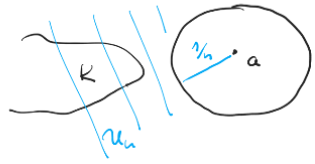
\includegraphics[width=0.5\linewidth]{figures/kompakt_abgeschlossen_beweis}
            \label{fig:kompakt_abgeschlossen_beweis}
        \end{figure}
        \( U_n\) ist offen (denn \( X\setminus U_n=\overline{B_{1/n}(a)}\)) und \( \bigcup_{n=1}^{\infty}U_n=X\setminus \Set{a}\supset K\).
        \( K\) kompakt \timplies \texists \( U_{n_1},\ldots, U_{n_L}\) \sd \( K\subset U_{n_1}\cup \cdots \cup U_{n_l}\). Setze \( N\definedas \max\Set{n_1,\ldots,n_l}\). Dann ist \( B_{\frac{1}{N}}(a)\subset X\setminus K\) \timplies \( X\setminus K \) ist offen \timplies \Beh.
        
        \item[Beschränktheit:] Sei \( a\in X\). Dann ist \( X=\bigcup\limits_{n=1}^{\infty} B_n(a) \) und somit \( (B_n(a))_n\) eine offene Überdeckung von \( K\).
        \begin{align*}
            \implies &\exists n_1,\ldots, n_k\logicspace  \sd\logicspace  K\subset B_{n_1(a)}\cup \cdots B_{n_k}(a)\\
            \implies &K\subset B_N(a) \text{ für }N=\max\Set{n_1,\ldots,n_k}\\
            \implies &\diam(K)\leq 2N.
        \end{align*}     
    \end{proofdescription}    
\end{proof}
\begin{folgerung*}
    Konvergente Folgen sind beschränkt.
\end{folgerung*}
\begin{bemerkung*}
    Die Umkehrung von \ref{kompakt:abgeschlossen_beschraenkt} gilt im Allgemeinen nicht!
    
    \( (X,d_{\text{discrete}})\), \( X\) habe unendlich viele Elemente. Jede Teilmenge ist abgeschlossen (da jede offen ist) und beschränkt (durch \( 1\)), aber nur die \emph{endlichen} sind kompakt.
\end{bemerkung*}
\begin{lemma}\label{abgeschlossene_teilmenge_kompakter_menge_ist_kompakt}
    Ist \( K\subset X\) kompakt und \( A\subset K\) ist abgeschlossen, so ist \( A\) kompakt.
\end{lemma}
\begin{proof}
    Sei \( (U_j)_j\) offene Überdeckung von \( A\). Es ist
    \begin{align*}
        &(\underbrace{X\setminus A}_{\mathclap{\text{offen (VOR)}}})\cup \bigcup U_j=X\supset K\\
        \implies &\exists j_1,\ldots, j_L\logicspace \sd\logicspace K\subset (X\setminus A)\cup U_{j_1}\cup \cdots \cup U_{j_L}\\
        \implies &A\subset U_{j_1}\cup \cdots \cup U_{j_L}.  
    \end{align*}
    
\end{proof}


\begin{satz}\label{kompakte_menge_stetiges_bild_kompakt}
    Seien \( X,Y\) metrische Räume und \( f\maps X\to Y\) stetig. Ist \( K\subset X\) kompakt, so ist auch \( f(K)\subset Y\) kompakt. 
\end{satz}
\begin{proof}
    Sei \( (U_j)_j\) offene Überdeckung von \( f(K)\). \( f\) stetig \( \underset{\ref{stetigkeit_in_topologischen_raeumen:urbildkriterium}}{\implies}\) Die Urbilder \( V_j \definedas \inv{f}(U_j)\) sind offen.
    
    Und nach Definition ist \( K\subset \bigcup_j V_j\).
    \begin{align*}
        \underset{\text{VOR}}{\implies} \exists j_1,\ldots, j_N\sd K\subset V_{j_1}\cup \cdots \cup V_{j_N}\\
        \implies f(K)\subset U_{j_1}\cup \cdots\cup U_{j_N}.
    \end{align*} 
    
\end{proof}

\begin{satz}\label{funktion_von_kompaktem_metrischen_raum_zu_r_kriegt_min_max}
    Sei \( \mathfrak{X}\) kompakter metrischer Raum, \( f\maps \mathfrak{X}\to \reals \) stetig. Dann ist \( f\) beschränkt und nimmt ihr Maximum und Minimum an, \dh \texists \( a,b \in \mathfrak{X}\)
    \begin{align*}
        f(a)=\sup\Set{f(x)|x\in \mathfrak{X}},\quad f(b)=\inf\Set{f(x)|x\in \mathfrak{X}}.
    \end{align*} 
\end{satz}
\begin{proof}
    \ref{kompakte_menge_stetiges_bild_kompakt} \timplies \( f(\mathfrak{X})\) ist kompakt. Mit \ref{kompakt:abgeschlossen_beschraenkt} folgt: \( f(\mathfrak{X})\) ist beschränkt (somit ist \( f\) beschränkt) und abgeschlossen.
    
    Also sind \( \sup f(\mathfrak{X})\) und \( \inf(\mathfrak{X})\) endlich. Zudem gibt es
    \begin{align*}
        (y_k)_k &\subset f(\mathfrak{X}),\quad y_k\goesto \sup(f(\mathfrak{X}))\\
        (z_k)_k\subset f(\mathfrak{X}), \quad z_k\goesto \inf(\mathfrak{X}),
    \end{align*}
    somit (Abgeschlossenheit!)
    \begin{align*}
        \sup(f(\mathfrak{X}))\in f(\mathfrak{X})\\
        \inf(f(\mathfrak{X}))\in f(\mathfrak{X})
    \end{align*}
    \timplies \Beh.
\end{proof}

\begin{beispiel*}
    Sei \( (\mathfrak{X},d)\) metrischer Raum. \( M\subset \mathfrak{X}\). Sei \( x\in \mathfrak{X}\). Der \emph{Abstand} von \( a\) zu \( M\) ist definiert als
    \begin{align*}
        \dist(x,M)\definedas \inf\Set{d(x,y)|y\in M}.
    \end{align*} 
    \begin{behauptung*}
        \( x\mapsto \dist(x,M)\) ist stetig auf \( \mathfrak{X}\). 
    \end{behauptung*}
    \begin{proof}
        Sei \( \varepsilon>0\). Dann ist
        \begin{align*}
            \abs{\dist(x,M)-\dist(\tilde{x},M)}\leq d(x,\tilde{x})<\varepsilon \quad \text{falls }d(x,\tilde{x})<\varepsilon, 
        \end{align*}
        denn
        \begin{align*}
            \dist(x,M)\underset{\triangle}{\leq}d(x,\tilde{x})+\dist(\tilde{x},M)\quad \forall x,\tilde{x}\in \mathfrak{X}.
        \end{align*}
        
    \end{proof}
    Definiere zu \( K\subset \mathfrak{X} \)
    \begin{align*}
        \dist(K,M)\definedas \inf\Set{\dist(x,M)|x\in K}.
    \end{align*}
    \begin{behauptung*}
        Ist \( M \) abgeschlossen, \( K \) kompakt und ist \( M\cap K=\emptyset \), so gilt \( \dist(M,K)>0 \).
    \end{behauptung*}
    \begin{proof}
        \( x\mapsto \dist(x,M) \) ist stetig auf \( \mathfrak{X} \), somit erst recht auf \( K \). \( K \) ist kompakt \( \overset{\ref{funktion_von_kompaktem_metrischen_raum_zu_r_kriegt_min_max}}{\implies} \) \texists \( a\in K \) \sd \( \dist(a,M)=\dist(K,M) \). \( M \) abgeschlossen \timplies \texists \( \varepsilon>0 \) \sd \( B_{\varepsilon}(a)\subset X\setminus K \) \timplies \( \dist(a,M)\geq \varepsilon \).
        
    \end{proof}
    \begin{achtung*}
        \begin{enumerate}
            \item Betrachte
            \begin{align*}
                M=\Set{(x,y)|xy=0}\subset , N=\set{(x,y)|xy=1}\subset \reals^2\\
                \dist(M,N)=0.
            \end{align*}
            \begin{figure}[H]
                \centering
                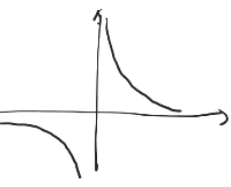
\includegraphics[width=0.3\linewidth]{figures/achsen_und_eins_durch_x}
                \caption*{}
                \label{fig:achsen_und_eins_durch_x}
            \end{figure}
            
            \item Betrachte \( B_{1/2}(1) \), \( B_{1/2}(2)\subset \reals^2 \), \( d_{\text{Euklidisch}} \). Distanz ist \( 0 \).
            \begin{figure}[H]
                \centering
                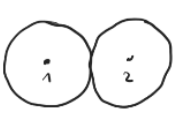
\includegraphics[width=0.3\linewidth]{figures/beruehrende_kreise}
                \label{fig:beruehrende_kreise}
            \end{figure}
            
        \end{enumerate}
    \end{achtung*}    
\end{beispiel*}
\begin{satzdef}
    Seien \( \mathfrak{X},Y \) metrische Räume, \( \mathfrak{X} \) kompakt. Dann ist jede stetig Abbildung \( f\maps \mathfrak{X}\to Y \) sogar \emph{gleichmäßig stetig} \dh im \( \varepsilon \)-\( \delta \)-Kriterium kann \( \delta \) unabhängig von \( x \) gewählt werden:
    \begin{align*}
        \forall \varepsilon>0\logicspace \exists \delta>0\logicspace \sd\logicspace d_Y(f(x),f(\tilde{x}))<\varepsilon\quad \forall x,\tilde{x},d_{\mathfrak{X}}(x,\tilde{x})<\delta.
    \end{align*}
\end{satzdef}
\begin{proof}
    Sei \( \varepsilon>0 \). Dann gibt es zu \( a\in \mathfrak{X} \) ein \( \delta(a)>0 \) \sd
    \begin{align*}
        d_Y(f(a),f(y))<\varepsilon\quad \forall y\in B_{\delta(a)}(a).
    \end{align*}
    Es gilt \( \bigcup_{a\in X} B_{\frac{\delta(a)}{2}}(a)=\mathfrak{X}\).

    \( \mathfrak{X} \) ist kompakt \timplies \texists \( a_1,\ldots,a_N \) \sd \( X=\bigcup\limits_{j=1}^{N}B_{\delta(a_j)/2} (a_j)\). Setze 
    \begin{align*}
        \delta\definedas \frac{1}{2}\min\Set{\delta(a_1),\ldots,\delta(a_N)}.
    \end{align*}

    Seien jetzt \( x,\tilde{x} \) beliebig aus \( \mathfrak{X} \) mit \( d_{\mathfrak{X}}(x,\tilde{x})<\delta \). Dann gibt es ein \( j\in \Set{1,\ldots, N} \) \sd \( x\in B_{\delta(a_j)/2} \) und somit \( \tilde{x}\in B_{\delta(a_j)}(a_j) \)
    \begin{align*}
        \implies &d_Y(f(x),f(a_j))<\varepsilon \quad d_Y(f(\tilde{x}),f(a_j))<\varepsilon\\
        \implies &d_Y(f(x),f(\tilde{x}))<2\varepsilon \quad \forall x,\tilde{x},\logicspace d_{\mathfrak{X}}(x,\tilde{x})<\delta.
    \end{align*}
    \begin{figure}[H]
        \centering
        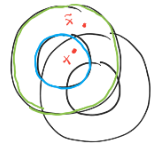
\includegraphics[width=0.4\linewidth]{figures/doppel_doppel_ball}
        \label{fig:doppel_doppel_ball}
    \end{figure}
    
\end{proof}
\begin{satz}[Bolzano-Weierstraß]\label{bolzanoweierstrass}
    Sei \( (X,d) \) metrischer Raum. Sei \( K\subset X \) kompakt. Dann besitzt jede Folge \( (x_n)_n \) in \( K \) eine Teilfolge \( (x_{n_k})_k \), die gegen einen Punkt \( x\in K \) konvergiert. 
\end{satz}
\begin{proof}
    Angenommen, \tnexists Teilfolge, die gegen einen Punkt von \( K \) konvergiert. Dann besitzt jedes \( x\in K \) eine offene Umgebung \( U_x \), in der nur endlich viele Folgenglieder liegen (sonst könnte man eine gegen \( x \) konvergente Teilfolge konstruieren). Es gilt: \( \bigcup_{x\in K}U_x\supset K \)
    \begin{align*}
        \implies \exists x_1,\ldots, x_N\logicspace \sd \logicspace \bigcup_{j=1}^{N}U_{x_j}\subset K   
    \end{align*}
    Aber dann liegen nur endlich viele \( x_k \) in \( K \), \contra zur Definition.
    
\end{proof}



